%%%%%%%%%%%%%%%%%%%%%%%%%%%%%%%%%%%%%%%%%%%%%%%%%%%%%%%%%%%%%%%%%%%%
%% I, the copyright holder of this work, release this work into the
%% public domain. This applies worldwide. In some countries this may
%% not be legally possible; if so: I grant anyone the right to use
%% this work for any purpose, without any conditions, unless such
%% conditions are required by law.
%%%%%%%%%%%%%%%%%%%%%%%%%%%%%%%%%%%%%%%%%%%%%%%%%%%%%%%%%%%%%%%%%%%%

\documentclass{beamer}
\usetheme[faculty=fi]{fibeamer}
\usepackage[utf8]{inputenc}
\usepackage[
  main=english, %% By using `czech` or `slovak` as the main locale
                %% instead of `english`, you can typeset the
                %% presentation in either Czech or Slovak,
                %% respectively.
  czech, slovak %% The additional keys allow foreign texts to be
]{babel}        %% typeset as follows:
%%
%%   \begin{otherlanguage}{czech}   ... \end{otherlanguage}
%%   \begin{otherlanguage}{slovak}  ... \end{otherlanguage}
%%
%% These macros specify information about the presentation
\title{Use of Transactions within a Reactive Microservices Environment} %% that will be typeset on the

\author{Bc. Martin Štefanko}
%% These additional packages are used within the document:
\usepackage{ragged2e}  % `\justifying` text
\usepackage{booktabs}  % Tables
\usepackage{tabularx}
\usepackage{tikz}      % Diagrams
\usetikzlibrary{calc, shapes, backgrounds}
\usepackage{amsmath, amssymb}
\usepackage{listings}  % Code listings
\usepackage{hyperref}
\frenchspacing
\begin{document}
  \frame{\maketitle}
    
    \begin{frame}{Assignment}
        \begin{itemize}
            \item Review the state of the art, in terms of problems of synchronous/blocking approaches for transaction management and other approaches/patterns available - taking into account the microservices context
            
            \item Propose a proof-of-concept implementation, using the Narayana transaction manager and prepare a service capable to manage transactions in the context of reactive microservices
            
            \item Prepare an example/quickstart showing the whole issues in more practical terms, proving that the transaction manager can work in an asynchronous environment
        \end{itemize}
    
    \end{frame}   
     
    \begin{frame}{Microservices}
    
        \begin{tikzpicture}
        \node  {
            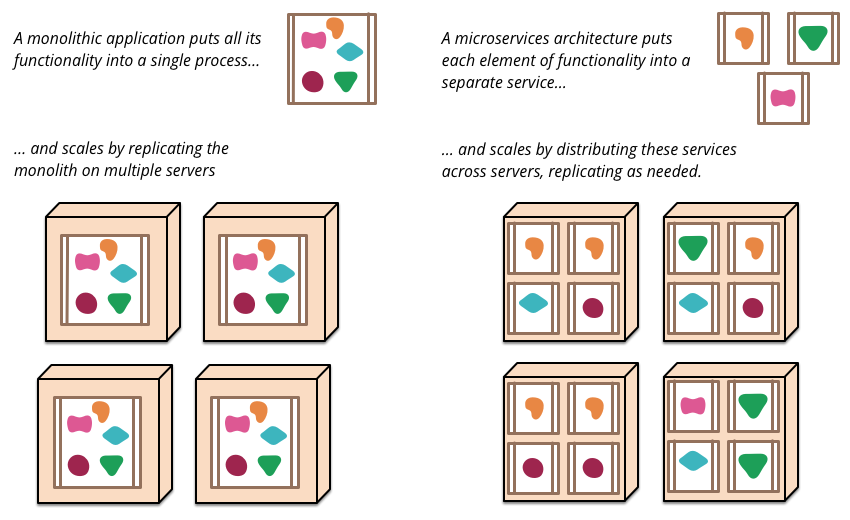
\includegraphics[width=100mm]{resources/fowlerMS.png}
        };
        \end{tikzpicture}%
    
    \end{frame}

    \begin{frame}{Reactive microservices}
       \begin{itemize}
           \item reactive systems
           \item reactive programming
           \item reactive streams
       \end{itemize}
     \begin{tikzpicture}[overlay]
    \node[anchor=south east,xshift=-50pt,yshift=-80pt]
    at (current page.south east) {
        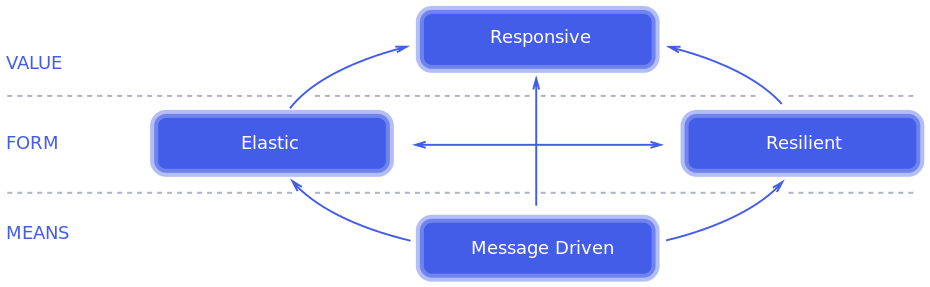
\includegraphics[width=85mm]{resources/reactive-traits.png}
    };
    \end{tikzpicture}%
    \hfill \break
    \hfill \break
    \hfill \break
    \hfill \break
    \hfill \break
    \hfill \break
    \hfill \break
    \end{frame}

    \begin{frame}{Transactions}
    
     \begin{quotation}
         \begin{center}
             "A transaction is a unit of processing that provides all-or-nothing property to the work that is conducted within its scope, also ensuring thatshared resources are protected from multiple users" \cite{java_transaction_processing}.
         \end{center}
     \end{quotation}
     \Large
        \begin{itemize}
            \item sequence of operations
            \item commit or rollback
        \end{itemize}
        \begin{tikzpicture}[overlay]
        \node[anchor=south east,xshift=-50pt,yshift=-40pt]
        at (current page.south east) {
            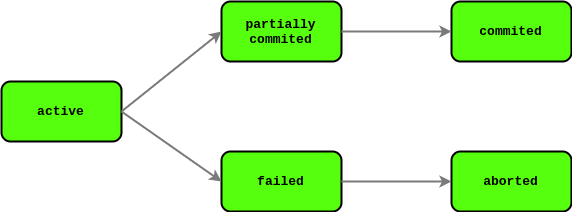
\includegraphics[width=65mm]{resources/transaction_states.png}
        };
        \end{tikzpicture}%
        \hfill \break
        \hfill \break
        
    \end{frame}
    
\begin{frame}{ACID transaction}

    \Large
    \begin{itemize}
        \item Atomicity
        \item Consistency
        \item Isolation
        \item Durability
    \end{itemize}
    \begin{tikzpicture}[overlay]
    \node[anchor=south east,xshift=-70pt,yshift=-50pt]
    at (current page.south east) {
        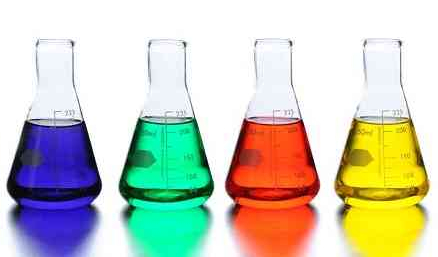
\includegraphics[width=55mm]{resources/vials.jpg}
    };
    \end{tikzpicture}%
    \hfill \break
    \hfill \break
    \hfill \break

\end{frame}

\begin{frame}{Distributed transactions}

    \begin{itemize}
        \item XA 
        \begin{tikzpicture}[overlay]
        \node[anchor=south east,xshift=-150pt,yshift=-75pt]
        at (current page.south east) {
            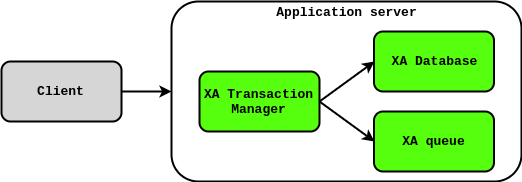
\includegraphics[width=70mm]{resources/XATransaction.png}
        };
        \end{tikzpicture}%
        \hfill \break
        \hfill \break
        \hfill \break
        \hfill \break
        \hfill \break
        \item Distributed system
        \begin{tikzpicture}[overlay]
        \node[anchor=south east,xshift=-230pt,yshift=-75pt]
        at (current page.south east) {
            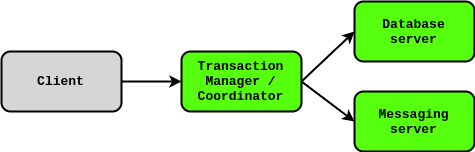
\includegraphics[width=65mm]{resources/DistributedTransaction.png}
        };
        \end{tikzpicture}%
        
        \hfill \break
        \hfill \break
        \hfill \break
        \hfill \break
        \hfill \break
    \end{itemize}

\end{frame}

\begin{frame}{Two phase commit protocol}

\hfill \break
\hfill \break
\hfill \break
\hfill \break
\hfill \break
\Large
\begin{itemize}
    \item $O(n^2)$ messages
    \item blocking
    \item coordinator - single point of failure
\end{itemize}
\begin{tikzpicture}[overlay]
\node[anchor=south east,xshift=-40pt,yshift=65pt]
at (current page.south east) {
    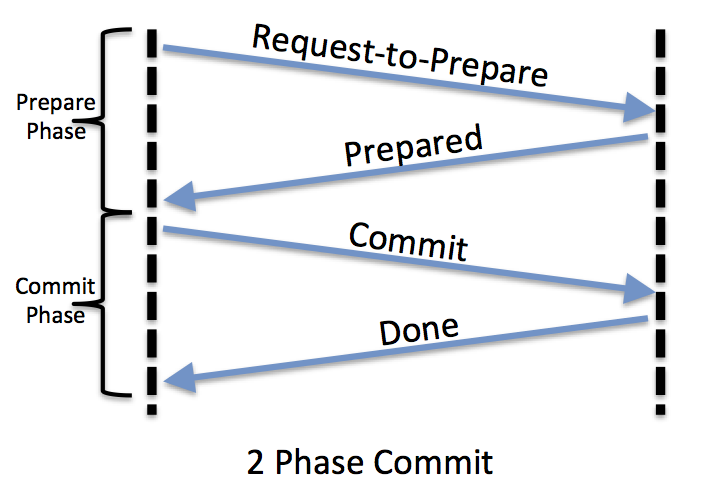
\includegraphics[width=65mm]{resources/2pc-seq.png}
};
\end{tikzpicture}%

\end{frame}

\begin{frame}{Saga pattern}

\begin{quotation}
\begin{center}
    Hector Garcia-Molina and Kenneth Salem, Princeton University, 1987
\end{center}
\end{quotation}

\Large
\begin{itemize}
    \item long lived transactions
    \item compensations
    \item all-or-nothing property
\end{itemize}

\end{frame}


\begin{frame}{Saga executions}

\Large
\begin{itemize}
    \item 2PC - $T_1$, $T_2$, ..., $T_n$ (in a single step)
    \item Saga
    \begin{itemize}
        \Large
        \item success - $T_1$, $T_2$, ..., $T_n$
        \item failure - $T_1$, $T_2$, ..., $T_k$, $C_k$, $C_{k-1}$, ..., $C_1$
    \end{itemize}
\end{itemize}

\end{frame}

\begin{frame}{BASE transaction}
    \Large
    \begin{itemize}
        \item Basically Available
        \item Soft state
        \item Eventual consistency
    \end{itemize}
\begin{tikzpicture}[overlay]
\node[anchor=south east,xshift=-50pt,yshift=-80pt]
at (current page.south east) {
    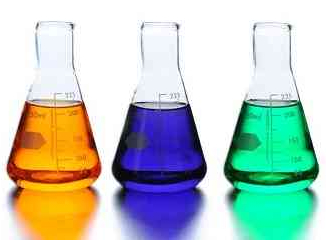
\includegraphics[width=55mm]{resources/base1.jpg}
};
\end{tikzpicture}%
\hfill \break
\hfill \break
\hfill \break
\hfill \break

\end{frame}

\begin{frame}{Two phase commit protocol}

\begin{tikzpicture}[overlay]
\node[anchor=south east,xshift=-50pt,yshift=-105pt]
at (current page.south east) {
    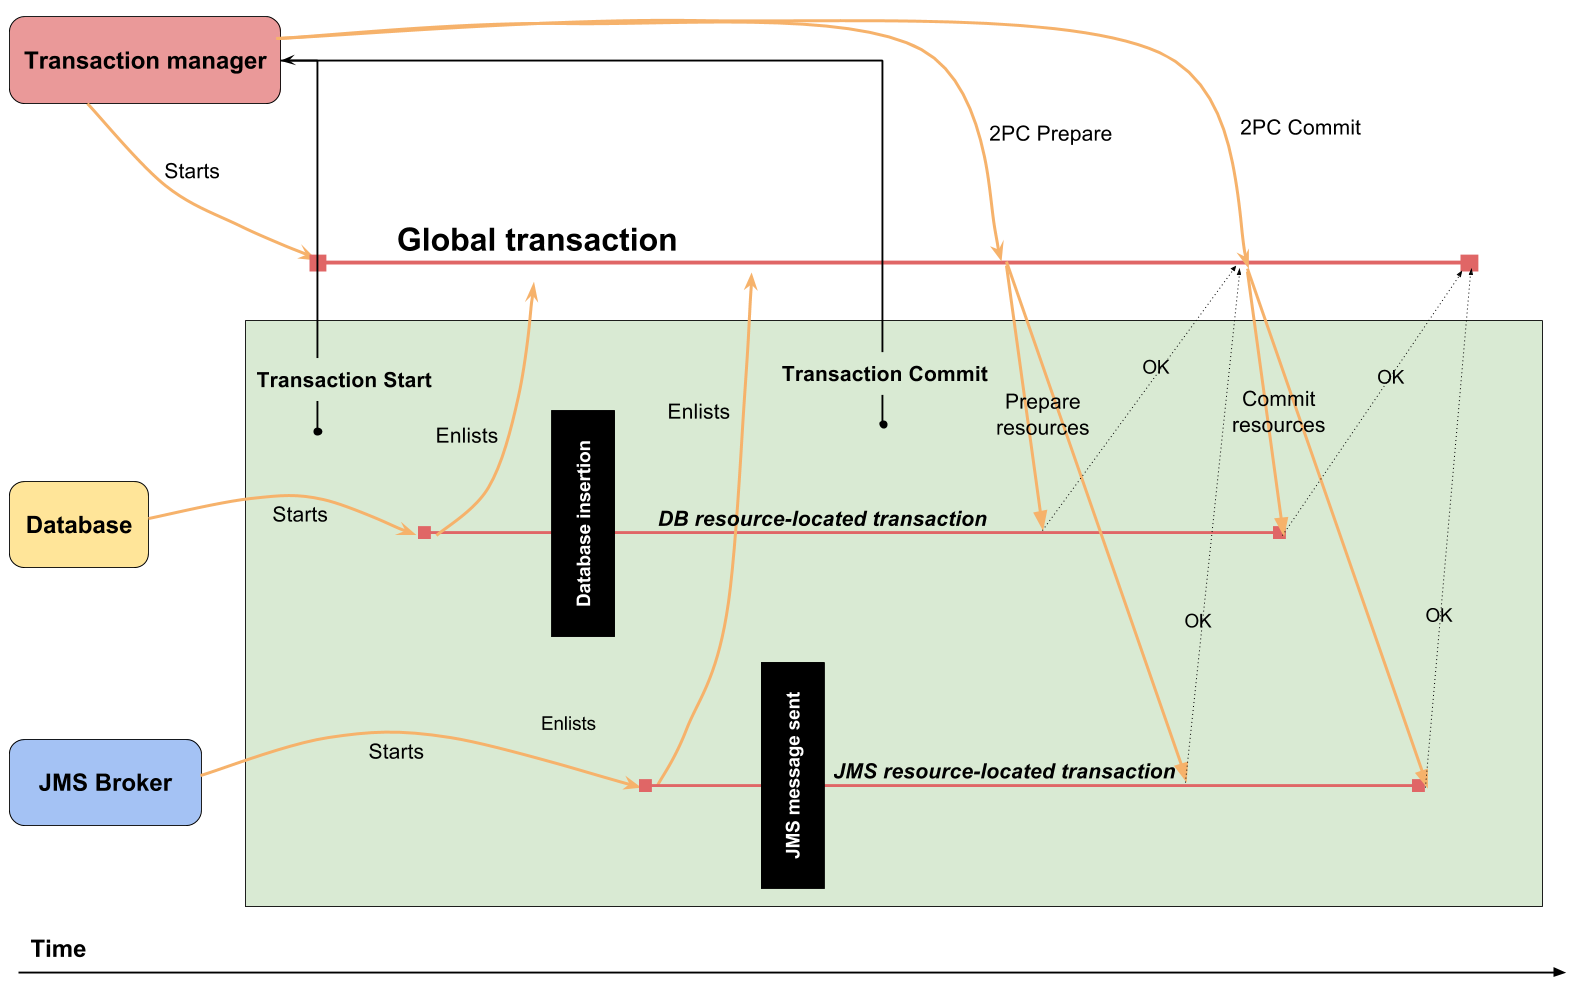
\includegraphics[width=110mm]{resources/2pc.png}
};
\end{tikzpicture}%

\end{frame}

\begin{frame}{Saga pattern}

\begin{tikzpicture}[overlay]
\node[anchor=south east,xshift=-40pt,yshift=-115pt]
at (current page.south east) {
    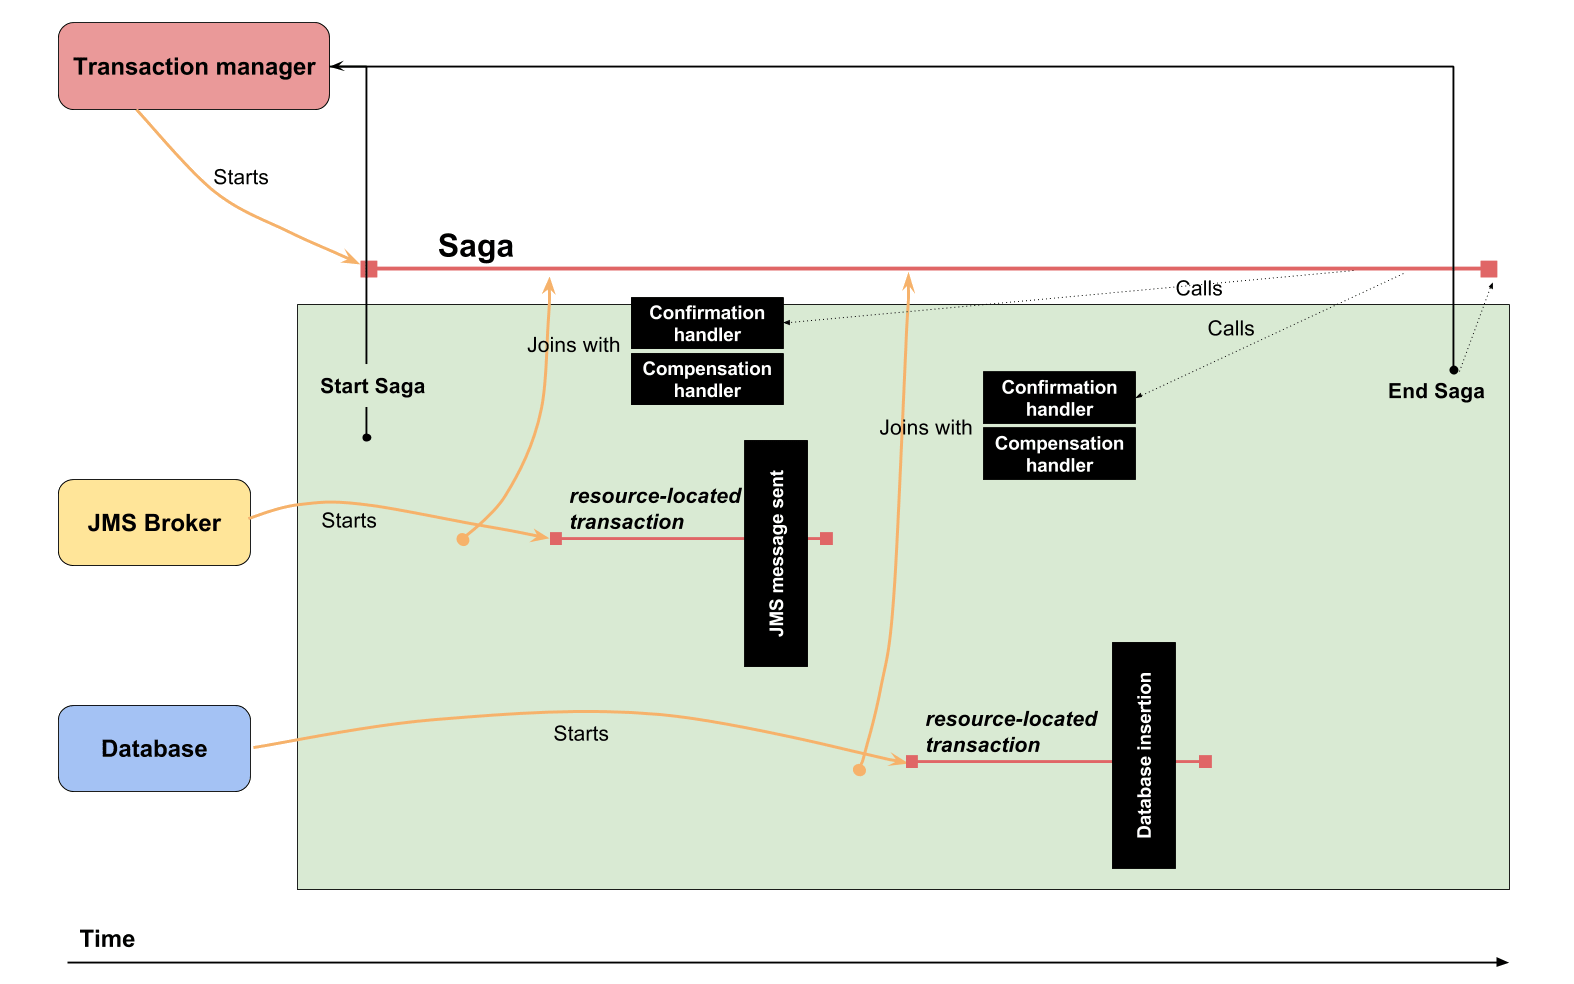
\includegraphics[width=117mm]{resources/saga.png}
};
\end{tikzpicture}%

\end{frame}

\begin{frame}{Saga implementations comparison scenario}

\begin{tikzpicture}[overlay]
\node[anchor=center,xshift=-35pt,yshift=0pt]
at (current page.south) {
    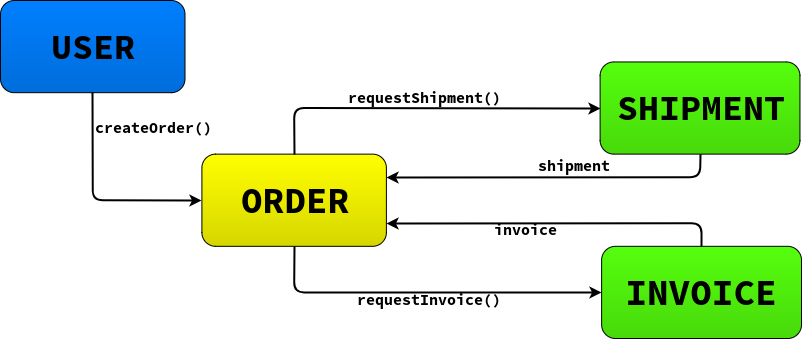
\includegraphics[width=100mm]{resources/SagaModel.png}
};
\end{tikzpicture}%

\end{frame}

\begin{frame}{Saga implementations investigation}

\Large
\begin{itemize}
    \item Axon framework
    \item Eventuate Event Sourcing (ES)
    \item Eventuate Tram
    \item Narayana Long Running Actions (LRA)
\end{itemize}

\end{frame}

\begin{frame}{Saga implementations comparison}

\begin{tikzpicture}[overlay]
\node[anchor=center,xshift=-35pt,yshift=0pt]
at (current page.south) {
    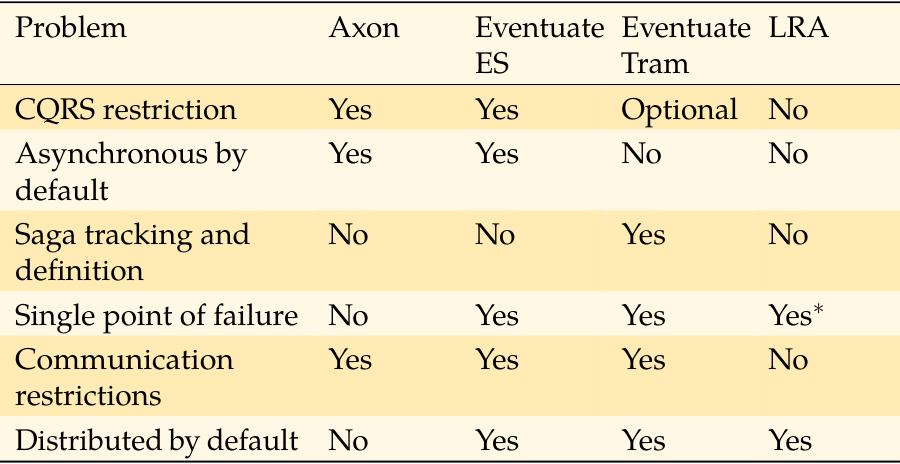
\includegraphics[width=110mm]{resources/comparison.png}
};
\end{tikzpicture}%


\end{frame}

\begin{frame}{Saga implementations performance testing}

\Large
\begin{itemize}
    \item Axon - 2 reported issues
    \item Eventuate ES - 1 reported issue
    \item Eventuate Tram - 1 feature request
    \item Narayana LRA
\end{itemize}

\end{frame}

\begin{frame}{LRA executor motivation}

\begin{tikzpicture}[overlay]
\node[anchor=center,xshift=-35pt,yshift=0pt]
at (current page.south) {
    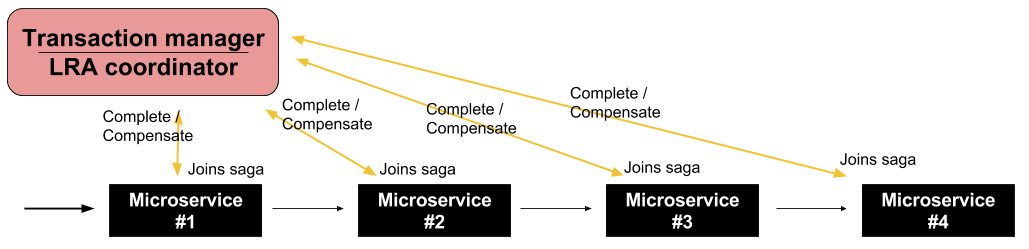
\includegraphics[width=110mm]{resources/msa_calls.png}
};
\end{tikzpicture}%


\end{frame}

\begin{frame}{LRA executor extension}

\begin{itemize}
    \item proof of concept / prototype
    \item asynchronous
    \item extensible and flexible design
    \item protocol / platform independent
    \begin{itemize}
        \item further future extensions are expected
    \end{itemize}
    \item two modules
    \begin{itemize}
        \item LRA definitions
        \item LRA executor
    \end{itemize}
\end{itemize}


\end{frame}

\begin{frame}{LRA Definitions}

\begin{itemize}
    \item \texttt{LRADefinition}
    \item \texttt{Action}
    \item fluent API
\end{itemize}

\begin{tikzpicture}[overlay]
\node[anchor=center,xshift=-110pt,yshift=-40pt]
at (current page.south) {
    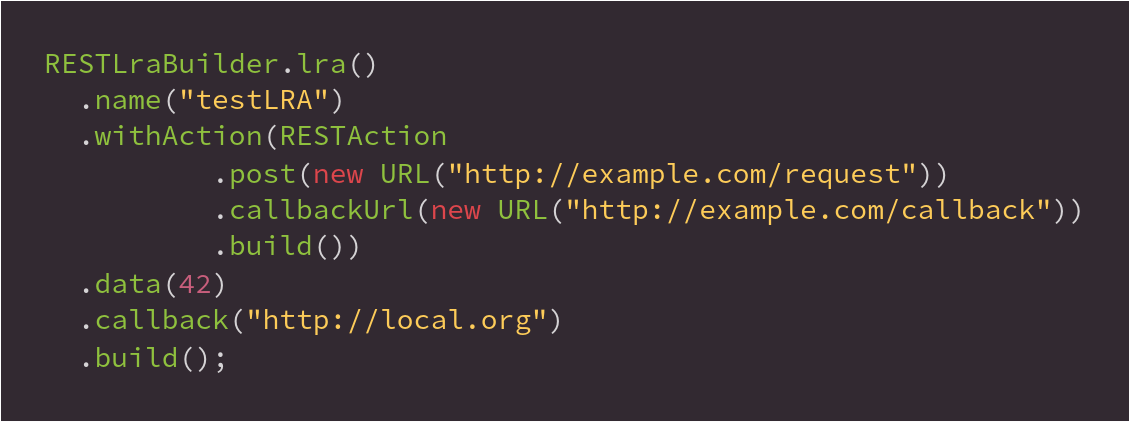
\includegraphics[width=60mm]{resources/restDef.png}
};
\end{tikzpicture}%

\begin{tikzpicture}[overlay]
\node[anchor=center,xshift=60pt,yshift=-25pt]
at (current page.south) {
    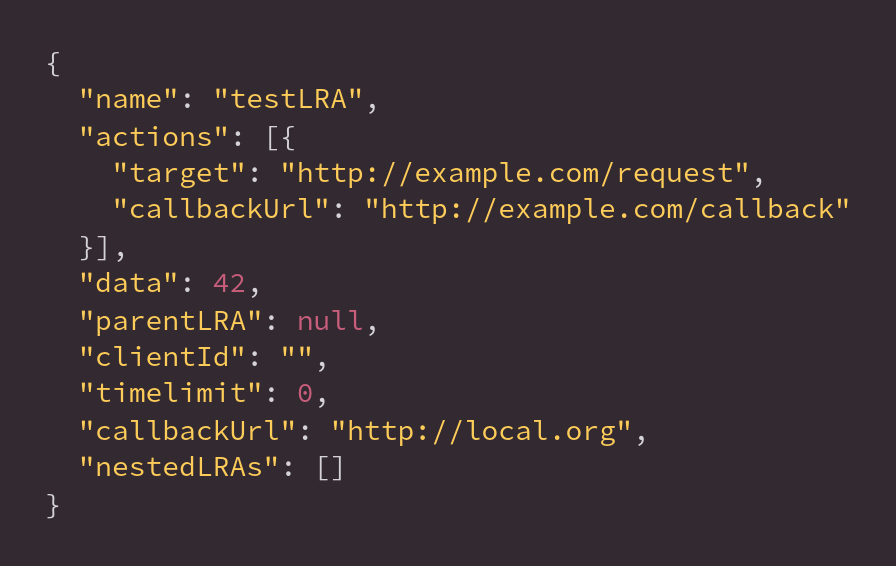
\includegraphics[width=50mm]{resources/carbon.png}
};
\end{tikzpicture}%

\hfill \break
\hfill \break
\hfill \break
\hfill \break
\hfill \break
\hfill \break

\end{frame}

\begin{frame}{LRA executor}

\begin{itemize}
    \item \texttt{LRAExecutor}
    \item synchronous and asynchronous executions
    \item \texttt{AbstractLRAExecutor} -- default implementation
    \begin{itemize}
        \item actions are invoked in the declared order
    \end{itemize}
    \item LRA manipulation methods
    \begin{itemize}
        \item startLRA, completeLRA, compensateLRA
    \end{itemize}
    \item integrated and tested (quickstart) with Narayana 5.8.1.Final
\end{itemize}


\end{frame}

\begin{frame}{Future work}

\begin{itemize}
    \item integration in the Narayana codebase
    \item communication methods 
    \item definition representations
    \item processing strategies
\end{itemize}

\end{frame}

\begin{frame}{Questions}

\end{frame}

\begin{frame}[label=bibliography]{Bibliography}
    \begin{thebibliography}{9}
        \bibitem{java_transaction_processing}
        M.~Little, J.~Maron, and G.~Pavlik.
        \emph{Java transaction processing}.
        Prentice Hall, 2004.
        \bibitem{lamport94}
        Leslie~Lamport.
        \emph{\LaTeX : A Document Preparation System}.
        Addison-Wesley, 1986.
        \bibitem{MG94}
        M.~Goossens, F.~Mittelbach, and A.~Samarin.
        \emph{The \LaTeX\ Companion}.
        Addison-Wesley, 1994.
        \bibitem{tantau04}
        Till~Tantau.
        \emph{User's Guide to the Beamer Class Version 3.01}.
        Available at \url{http://latex-beamer.sourceforge.net}.

        \bibitem{fowlerMS}
        \small
        \href{https://www.martinfowler.com/articles/microservices.html}{https://www.martinfowler.com/articles/microservices.html}
        \bibitem{vials}
        \href{http://www.24pressrelease.com/assets/news/Propylene\%20Glycol\%20Solvent\%2017614.jpg}{http://www.24pressrelease.com/assets/news/Propylene\\\%20Glycol\%20Solvent\%2017614.jpg}.
        \bibitem{2pc-seq}
        \href{https://encrypt.co.in/2-phase-commit-protocol/}{https://encrypt.co.in/2-phase-commit-protocol/}
    \end{thebibliography}


\end{frame}

\begin{frame}{Opponent's review}
    \Large
    \begin{itemize}
        \item transaction heuristic outcomes
        \begin{itemize}
            \item heuristic commit, rollback, mixed
            \item non-atomic outcome
            \item requires semantic knowledge
        \end{itemize}
        \item LRA service performance test
        \begin{itemize}
            \item REST requests queuing 
            %instead of the command sending in other frameworks
        \end{itemize}
        \item recovery capabilities of the executor
        \begin{itemize}
            \item main concern - failure after the marking of the participant invocation
            \item idempotent requests (may be too restrictive)
            \item timeouts
        \end{itemize}
    \end{itemize}
\end{frame}

\begin{frame}{Supervisor's review}
    \Large
    \begin{itemize}
        \item performance testing
        \item LRA specification relations
        \begin{itemize}
            \item still in the draft form
            \item focusing only on the coordination capabilities
            \item currently only providing the REST reference implementation
        \end{itemize}
    \end{itemize}
\end{frame}

\end{document}
